\section{The Fast Multipole Method}

The acceleration of the interpolation steps in the preceding section
relies on a sufficient accurate and optimized fast multipole method
(FMM) algorithm. The FMM is an algorithm which computes matrix-vector
products of a certain form in sub-quadratic
time~\cite{fmm-orig}. Typically, the FMM is developed for a particular
radial basis function of a certain dimensionality. In this work, we
provide an optimized one-dimensional FMM for the Cauchy kernel:
\begin{align}
  \label{eq:cauchy-kernel}
  \Phi(y, x) = \frac{1}{y - x}.
\end{align}
Implementing an FMM requires the derivation of regular and singular
factorizations the kernel function (so-called $S$-factorizations and
$R$-factorizations), along with derivations of translation operators
which reexpand these factorizations: singular-to-singular,
singular-to-regular, and regular-to-regular translation
operators~\cite{fmm-helmholtz}.

The $R$ and $S$-factorizations of the Cauchy kernel are derived in a
straightforward manner from the Taylor expansion of $\Phi$. For the
$S$-factorization, we fix $x, y$, and
$\xstar \suchthat \abs{x-\xstar} < \abs{y-\xstar}$ and define
$b_m(x, \xstar) = {(x - \xstar)}^m$ and
$S_m(y - \xstar) = {(y - \xstar)}^{-m-1}$. The point $\xstar$ is
referred to as the expansion center. Then, the $S$-factorization of
$\Phi$ is given by:
\begin{align}
  \label{eq:S-factorization}
  \Phi(y, x) = \sum_{m=0}^\infty b_m(x, \xstar) S_m(y - \xstar).
\end{align}
Very similarly, for the $R$-factorization, we fix $x, y$, and
$\xstar \suchthat \abs{y - \xstar} < \abs{x - \xstar}$ and define
$a_m(x, \xstar) = -{(x - \xstar)}^{-m-1}$ and
$R_m{(y - \xstar)}^m = {(y - \xstar)}^m$, giving us:
\begin{align}
  \label{eq:R-factorization}
  \Phi(y, x) = \sum_{m=0}^\infty a_m(x, \xstar) R_m(y - \xstar).
\end{align}
These expansions of $\Phi$ are used in the implementation of our FMM,
as well as in our discussion of error bounds.

The FMM involves evaluating a function which is comprised of a sum of
weighted kernels at a set of target points. In doing so, the
computational domain is decomposed using a spatial data structure
(e.g.\ a binary tree or octree). The algorithm first expands each
weighted kernel using an $S$-factorization, then applies the
translation operators according to the spatial decomposition
(Figure~\ref{fig:fmm}). We denote the singular-to-singular translation
matrix by $\SSmat$. Represented as an infinite matrix, its entries are
given by:
\begin{align}
  \label{eq:SSmat}
  \parens{\SSmat}_{n,m} \defd \frac{{(-1)}^{n-m} n! \delta^{n-m}}{(n-m)!m!},
\end{align}
where $\delta$ is the translation vector between the two expansion
centers. That is, if the resultant $S$-factorization is to be expanded
about $\xstar'$, then $\delta = \xstar - \xstar'$. The corresponding
$S$-reexpansion is:
\begin{align}
  \label{eq:SSmat-reexpansion}
  S_m(y - \xstar) = \sum_{n=0}^\infty \parens{\SSmat}_{n,m} S_n(y - \xstar').
\end{align}
Such a reexpansion requires that $\abs{\delta} < \abs{y -
  \xstar'}$. More details can be found in the appendix, but the
expressions for the singular-to-regular translation operator $\SRmat$
and the regular-to-regular translation operator $\RRmat$ are given by:
\begin{align}
  \label{eq:SRmat}
  \parens{\SRmat}_{n,m} \defd {\parens{-1}^n \parens{m + n}! \over m! n! \delta^{m+n+1}},
\end{align}
and:
\begin{align}
  \label{eq:RRmat}
  \parens{\RRmat}_{n,m} = \begin{cases}
    \frac{m! \delta^{m - n}}{(m - n)!n!} & \mbox{if } n \leq m, \\
    0 & \mbox{otherwise},
  \end{cases}
\end{align}
respectively.

\begin{figure}[h]
  \centering
  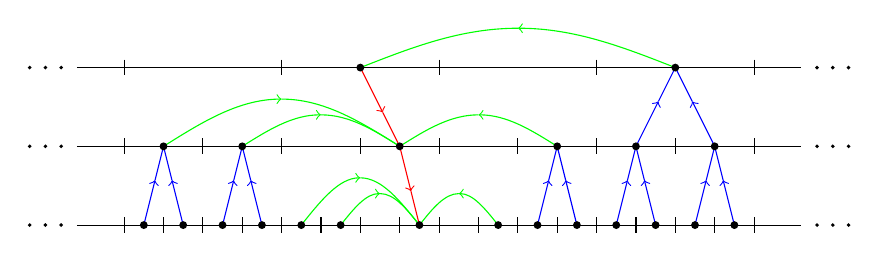
\begin{tikzpicture}[scale = 2.0]
  \def \cdotssizes{0.0125};
  \def \cdotspacing{0.1};
  \def \nodesize{0.025};
  \def \leftextent{0};
  \def \rightextent{4};
  \def \hmargin{0.3};
  \def \hrulertickheight{0.1};
  \def \yone {0.0};
  \def \ytwo {0.5};
  \def \ythree {1.0};
  \def \yfour {1.5};

  % Draw horizontal rulers and cdots on the sides.
  \foreach \y in {\yone, \ytwo, \ythree} {
    \draw [-] ({\leftextent - \hmargin}, \y) -- ({\rightextent + \hmargin}, \y);
    \foreach \i in {1, 2, 3} {
      \fill[black] ({\leftextent - \hmargin - (\i * \cdotspacing)}, \y) circle (\cdotssizes);
      \fill[black] ({\rightextent + \hmargin + (\i * \cdotspacing)}, \y) circle (\cdotssizes);
    }
  };
  
  % Draw ticks on each horizontal ruler.
  \foreach \x in {\leftextent, 1.0, ..., \rightextent} {
    \draw [-] (\x, {\ythree + (\hrulertickheight / 2)}) -- (\x, {\ythree - (\hrulertickheight / 2)});
  };
  \foreach \x in {\leftextent, 0.5, ..., \rightextent} {
    \draw [-] (\x, {\ytwo + (\hrulertickheight / 2)}) -- (\x, {\ytwo - (\hrulertickheight / 2)});
  };
  \foreach \x in {\leftextent, 0.25, ..., \rightextent} {
    \draw [-] (\x, {\yone + (\hrulertickheight / 2)}) -- (\x, {\yone - (\hrulertickheight / 2)});
  };
  
  % Draw SS translation arrows.
  \def \theta {4/7}
  \foreach \x in {0.25, 0.75, 2.75, 3.25, 3.75} {
    \def \midpt {(1 - \theta) * \yone + \theta * \ytwo};
    \draw [-, blue] (\x, \ytwo) -- ({\x - 0.125*(1 - \theta)}, {\midpt});
    \draw [<-, blue] ({\x - 0.125*(1 - \theta)}, {\midpt}) -- ({\x - 0.125}, \yone);
    \draw [-, blue] (\x, \ytwo) -- ({\x + 0.125*(1 - \theta)}, {\midpt});
    \draw [<-, blue] ({\x + 0.125*(1 - \theta)}, {\midpt}) -- ({\x + 0.125}, \yone);
  };
  \foreach \x in {3.5} {
    \def \midpt {(1 - \theta) * \ytwo + \theta * \ythree};
    \draw [-, blue] (\x, \ythree) -- ({\x - 0.25*(1 - \theta)}, {\midpt});
    \draw [<-, blue] ({\x - 0.25*(1 - \theta)}, {\midpt}) -- ({\x - 0.25}, \ytwo);
    \draw [-, blue] (\x, \ythree) -- ({\x + 0.25*(1 - \theta)}, {\midpt});
    \draw [<-, blue] ({\x + 0.25*(1 - \theta)}, {\midpt}) -- ({\x + 0.25}, \ytwo);
  };
  
  % Draw RR translation arrows.
  \def \theta {3/7}
  \foreach \x in {1.75} {
    \def \midpt {(1 - \theta) * \yone + \theta * \ytwo};
    \draw [->, red] (\x, \ytwo) -- ({\x + 0.125*(1 - \theta)}, {\midpt});
    \draw [-, red] ({\x + 0.125*(1 - \theta)}, {\midpt}) -- ({\x + 0.125}, \yone);
  };
  \foreach \x in {1.5} {
    \def \midpt {(1 - \theta) * \ytwo + \theta * \ythree};
    \draw [->, red] (\x, \ythree) -- ({\x + 0.25*(1 - \theta)}, {\midpt});
    \draw [-, red] ({\x + 0.25*(1 - \theta)}, {\midpt}) -- ({\x + 0.25}, \ytwo);
  };

  % Draw SR translation arrows.
  \def \center {1.5}
  \foreach \x in {3.5} {
    \pgfmathsetmacro{\xmid}{(\center + \x)/2};
    \pgfmathsetmacro{\ymid}{(\ythree + \yfour)/2};
    \draw[->, green] (\x, \ythree) sin (\xmid, \ymid);
    \draw[-, green] (\xmid, \ymid) cos (\center, \ythree);
  };
  \def \center {1.75}
  \pgfmathsetmacro{\maxdist}{abs(\center - 0.25)};
  \foreach \x in {0.25, 0.75, 2.75} {
    \pgfmathsetmacro{\dist}{abs(\center - \x)};
    \pgfmathsetmacro{\theta}{0.6 * \dist / abs(\maxdist)};
    \pgfmathsetmacro{\xmid}{(\center + \x)/2};
    \pgfmathsetmacro{\ymid}{(1 - \theta) * \ytwo + \theta * \ythree};
    \draw[->, green] (\x, \ytwo) sin (\xmid, \ymid);
    \draw[-, green] (\xmid, \ymid) cos (\center, \ytwo);
  };
  \def \center {1.875}
  \pgfmathsetmacro{\maxdist}{abs(\center - 1.125)};
  \foreach \x in {1.125, 1.375, 2.375} {
    \pgfmathsetmacro{\dist}{abs(\center - \x)};
    \pgfmathsetmacro{\theta}{0.6 * \dist / abs(\maxdist)};
    \pgfmathsetmacro{\xmid}{(\center + \x)/2};
    \pgfmathsetmacro{\ymid}{(1 - \theta) * \yone + \theta * \ytwo};
    \draw[->, green] (\x, \yone) sin (\xmid, \ymid);
    \draw[-, green] (\xmid, \ymid) cos (\center, \yone);
  };
  
  % Draw node circles.
  \foreach \x in {1.5, 3.5} {
    \fill[black] (\x, \ythree) circle (\nodesize);
  };
  \foreach \x in {0.25, 0.75, 1.75, 2.75, 3.25, 3.75} {
    \fill[black] (\x, \ytwo) circle (\nodesize);
  };
  \foreach \x in {0.125, 0.375, 0.625, 0.875, 1.125, 1.375, 1.875, 2.375, 2.625, 2.875, 3.125, 3.375, 3.625, 3.875} {
    \fill [black] (\x, \yone) circle (\nodesize);
  };
\end{tikzpicture} \\

%%% Local Variables:
%%% mode: latex
%%% TeX-master: "../paper/paper"
%%% End:

  \caption{an illustration of the translation phases of the
    one-dimensional FMM.}\label{fig:fmm}
\end{figure}

\begin{itemize}
\item \TODO\ redo style of TikZ plot using pgfplot colors/design.
\item \TODO\ truncations and error.
\item \TODO\ label translation operators in FMM figure, label direct
  sum bins vs far sum bins.
\item \TODO\ better colors for FMM figure.
\item \TODO\ make FMM figure breath a little better.
\end{itemize}

% Local Variables:
% TeX-master: "../paper.tex"
% indent-tabs-mode: nil
% End:
